% ===========================
%       Chapter 1A.4
%          Lipids
%   Created by Michael Tang
%        2024.12.30
% ===========================

\subsubsection{1A.4 \underline{Lipids} (脂类)}
\paragraph{Fats and Oils} Fats and oils are essential lipids with significant biological roles.
\begin{itemize}
    \item \textbf{Definition:} Lipids include fats and oil. Fats are solid at room temperature, while oils are liquid at room
    temperature.
    \item \textbf{Composition:}
    \begin{itemize}
        \item Made of \underline{glycerol} ($C_3H_8O_3$ 甘油) and fatty acids ($C_nH_{2n+1}COOH$ 脂肪酸).
        \begin{figure}[H]
            \centering
            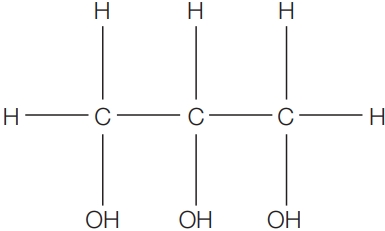
\includegraphics[scale=0.28]{Biology/1A/Images/1A-4-1.png}
            \caption{Displayed formula of glycerol (propane-1,2,3-triol).}
        \end{figure}
        \item Contain carbon ($C$), hydrogen ($H$), and small amount of oxygen ($O$) atoms.
    \end{itemize}
    \item \textbf{Sources:}
    \begin{itemize}
        \item \textbf{Fats:} \underline{Predominantly} (大多数情况下) from animal sources (e.g., butter, lard 猪油).
        \item \textbf{Oils:} Predominantly from plant sourcrs (e.g., olive oil, sunflower oil).
    \end{itemize}
    \item \textbf{Energy Content:}
    \begin{itemize}
        \item Store about three times as much energy as the same mass of carbohydrates.
        \item Act as long-term energy storage, especially in seeds and \underline{adipose tissue} (皮下脂肪组织).
    \end{itemize}
\end{itemize}

\paragraph{Fatty Acids} Fatty acids are hydrocarbon chains with a \underline{carboxyl group} ($-COOH$ 羧基) at one end.
\begin{itemize}
    \item \textbf{Types:}
    \begin{itemize}
        \item[1.] \textbf{\underline{Saturated Fatty Acids} (饱和脂肪酸):} Only single bonds between carbon atoms (e.g., stearic
        acid 硬脂酸).
        \begin{figure}[H]
            \centering
            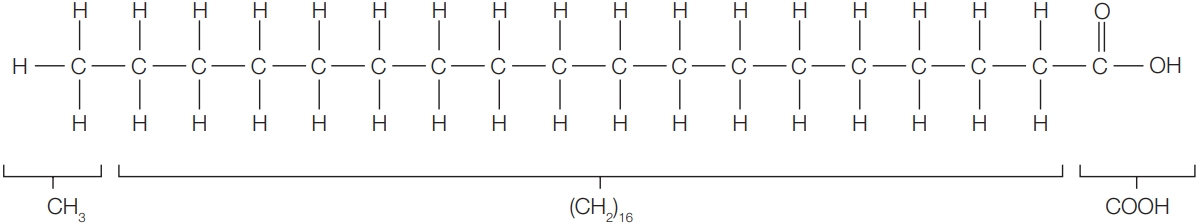
\includegraphics[scale=0.28]{Biology/1A/Images/1A-4-2.png}
            \caption{Displayed formula of stearic acid, a saturated fatty acid found in both plant and animal fats.}
        \end{figure}
        \item[2.] \textbf{\underline{Unsaturated Fatty Acids} (不饱和脂肪酸):}
        \begin{itemize}
            \item \textbf{\underline{Monounsaturated Fatty Acids} (单不饱和脂肪酸):} One double bond between carbon atoms.
            \item \textbf{\underline{Polyunsaturated Fatty Acids} (多不饱和脂肪酸):} Multiple carbon-carbon double bonds
            (e.g., linoleic acid 亚油酸).
        \end{itemize}
        \begin{figure}[H]
            \centering
            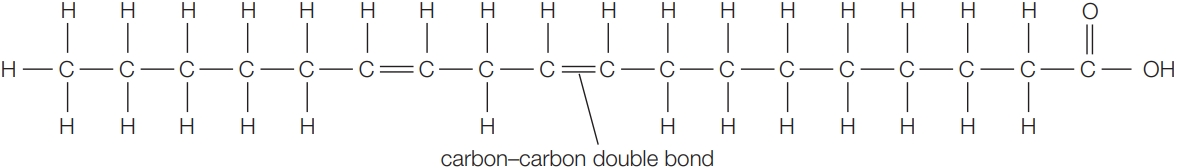
\includegraphics[scale=0.28]{Biology/1A/Images/1A-4-3.png}
            \caption{Displayed formula of linoleic acid, a polyunsaturated fatty acid.}
        \end{figure}
    \end{itemize}
    \item \textbf{Properties:}
    \begin{itemize}
        \item Saturated fats are more likely to be solid at room temperature.
        \item Unsaturated fats are usually liquid and healthier in the diet.
    \end{itemize}
\end{itemize}

\paragraph{Forming Ester Bonds} Ester bonds are formed in the synthesis of \underline{triglycerides} \footnote{Note that a
word with a prefix mono- usually means one, di- means two, tri- means three, and poly- means many.} (甘油三酯) through a
condensation reaction.
\begin{itemize}
    \item \textbf{Process:}
    \begin{itemize}
        \item[1.] \textbf{Reactants:}
        \begin{itemize}
            \item Glycerol provides hydroxyl groups ($-OH$).
            \item Fatty acids provide carboxyl groups ($-COOH$).
        \end{itemize}
        \item[2.] \textbf{Reaction:} A molecule of water ($H_2O$) is removed for each \underline{ester bond} \footnote{An ester
        bond is a covalent bond formed between the hydroxyl group ($-OH$) of glycerol and the carboxyl group ($-COOH$) of a fatty
        acid. This bond is a key structural feature of lipids, particularly triglycerides.} (酯键) formed.
        \item[3.] \textbf{Product:} One molecule of glycerol reacts with three fatty acids to form a triglyceride.
    \end{itemize}
    \item \textbf{Chemical Representation:}
    $$\text{Glycerol} + 3\text{Fatty Acids} \rightarrow \text{Triglyceride} + 3H_2O$$
    \item \textbf{Hydrolysis:} Ester bonds in triglycerides can be broken down by adding water, releasing glycerol and fatty
    acids.
    \begin{figure}[H]
        \centering
        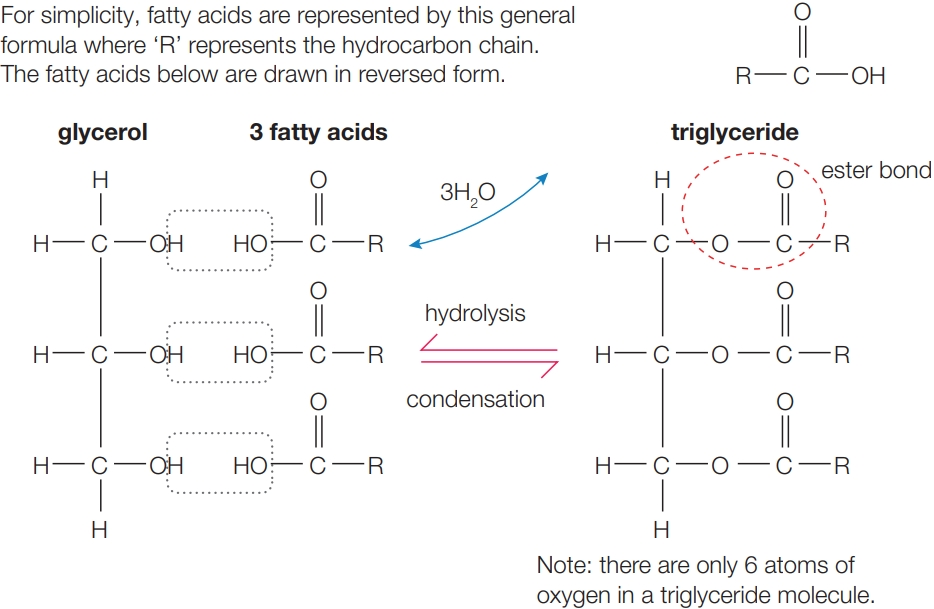
\includegraphics[scale=0.35]{Biology/1A/Images/1A-4-4.png}
        \caption{The formation of ester bonds.}
    \end{figure}
\end{itemize}